\PassOptionsToPackage{unicode=true}{hyperref} % options for packages loaded elsewhere
\PassOptionsToPackage{hyphens}{url}
%
\documentclass[english,man,floatsintext]{apa6}
\usepackage{lmodern}
\usepackage{amssymb,amsmath}
\usepackage{ifxetex,ifluatex}
\usepackage{fixltx2e} % provides \textsubscript
\ifnum 0\ifxetex 1\fi\ifluatex 1\fi=0 % if pdftex
  \usepackage[T1]{fontenc}
  \usepackage[utf8]{inputenc}
  \usepackage{textcomp} % provides euro and other symbols
\else % if luatex or xelatex
  \usepackage{unicode-math}
  \defaultfontfeatures{Ligatures=TeX,Scale=MatchLowercase}
\fi
% use upquote if available, for straight quotes in verbatim environments
\IfFileExists{upquote.sty}{\usepackage{upquote}}{}
% use microtype if available
\IfFileExists{microtype.sty}{%
\usepackage[]{microtype}
\UseMicrotypeSet[protrusion]{basicmath} % disable protrusion for tt fonts
}{}
\IfFileExists{parskip.sty}{%
\usepackage{parskip}
}{% else
\setlength{\parindent}{0pt}
\setlength{\parskip}{6pt plus 2pt minus 1pt}
}
\usepackage{hyperref}
\hypersetup{
            pdftitle={Automation-coerced, Increased Dilution of Correlation},
            pdfauthor={Chung-hong Chan1},
            pdfkeywords={Automated Content Analysis, Correlation Dilution, Measurement Error, Statistical Power},
            pdfborder={0 0 0},
            breaklinks=true}
\urlstyle{same}  % don't use monospace font for urls
\usepackage{color}
\usepackage{fancyvrb}
\newcommand{\VerbBar}{|}
\newcommand{\VERB}{\Verb[commandchars=\\\{\}]}
\DefineVerbatimEnvironment{Highlighting}{Verbatim}{commandchars=\\\{\}}
% Add ',fontsize=\small' for more characters per line
\usepackage{framed}
\definecolor{shadecolor}{RGB}{248,248,248}
\newenvironment{Shaded}{\begin{snugshade}}{\end{snugshade}}
\newcommand{\AlertTok}[1]{\textcolor[rgb]{0.94,0.16,0.16}{#1}}
\newcommand{\AnnotationTok}[1]{\textcolor[rgb]{0.56,0.35,0.01}{\textbf{\textit{#1}}}}
\newcommand{\AttributeTok}[1]{\textcolor[rgb]{0.77,0.63,0.00}{#1}}
\newcommand{\BaseNTok}[1]{\textcolor[rgb]{0.00,0.00,0.81}{#1}}
\newcommand{\BuiltInTok}[1]{#1}
\newcommand{\CharTok}[1]{\textcolor[rgb]{0.31,0.60,0.02}{#1}}
\newcommand{\CommentTok}[1]{\textcolor[rgb]{0.56,0.35,0.01}{\textit{#1}}}
\newcommand{\CommentVarTok}[1]{\textcolor[rgb]{0.56,0.35,0.01}{\textbf{\textit{#1}}}}
\newcommand{\ConstantTok}[1]{\textcolor[rgb]{0.00,0.00,0.00}{#1}}
\newcommand{\ControlFlowTok}[1]{\textcolor[rgb]{0.13,0.29,0.53}{\textbf{#1}}}
\newcommand{\DataTypeTok}[1]{\textcolor[rgb]{0.13,0.29,0.53}{#1}}
\newcommand{\DecValTok}[1]{\textcolor[rgb]{0.00,0.00,0.81}{#1}}
\newcommand{\DocumentationTok}[1]{\textcolor[rgb]{0.56,0.35,0.01}{\textbf{\textit{#1}}}}
\newcommand{\ErrorTok}[1]{\textcolor[rgb]{0.64,0.00,0.00}{\textbf{#1}}}
\newcommand{\ExtensionTok}[1]{#1}
\newcommand{\FloatTok}[1]{\textcolor[rgb]{0.00,0.00,0.81}{#1}}
\newcommand{\FunctionTok}[1]{\textcolor[rgb]{0.00,0.00,0.00}{#1}}
\newcommand{\ImportTok}[1]{#1}
\newcommand{\InformationTok}[1]{\textcolor[rgb]{0.56,0.35,0.01}{\textbf{\textit{#1}}}}
\newcommand{\KeywordTok}[1]{\textcolor[rgb]{0.13,0.29,0.53}{\textbf{#1}}}
\newcommand{\NormalTok}[1]{#1}
\newcommand{\OperatorTok}[1]{\textcolor[rgb]{0.81,0.36,0.00}{\textbf{#1}}}
\newcommand{\OtherTok}[1]{\textcolor[rgb]{0.56,0.35,0.01}{#1}}
\newcommand{\PreprocessorTok}[1]{\textcolor[rgb]{0.56,0.35,0.01}{\textit{#1}}}
\newcommand{\RegionMarkerTok}[1]{#1}
\newcommand{\SpecialCharTok}[1]{\textcolor[rgb]{0.00,0.00,0.00}{#1}}
\newcommand{\SpecialStringTok}[1]{\textcolor[rgb]{0.31,0.60,0.02}{#1}}
\newcommand{\StringTok}[1]{\textcolor[rgb]{0.31,0.60,0.02}{#1}}
\newcommand{\VariableTok}[1]{\textcolor[rgb]{0.00,0.00,0.00}{#1}}
\newcommand{\VerbatimStringTok}[1]{\textcolor[rgb]{0.31,0.60,0.02}{#1}}
\newcommand{\WarningTok}[1]{\textcolor[rgb]{0.56,0.35,0.01}{\textbf{\textit{#1}}}}
\usepackage{graphicx,grffile}
\makeatletter
\def\maxwidth{\ifdim\Gin@nat@width>\linewidth\linewidth\else\Gin@nat@width\fi}
\def\maxheight{\ifdim\Gin@nat@height>\textheight\textheight\else\Gin@nat@height\fi}
\makeatother
% Scale images if necessary, so that they will not overflow the page
% margins by default, and it is still possible to overwrite the defaults
% using explicit options in \includegraphics[width, height, ...]{}
\setkeys{Gin}{width=\maxwidth,height=\maxheight,keepaspectratio}
\setlength{\emergencystretch}{3em}  % prevent overfull lines
\providecommand{\tightlist}{%
  \setlength{\itemsep}{0pt}\setlength{\parskip}{0pt}}
\setcounter{secnumdepth}{0}

% set default figure placement to htbp
\makeatletter
\def\fps@figure{htbp}
\makeatother

% Manuscript styling
\usepackage{upgreek}
\captionsetup{font=singlespacing,justification=justified}

% Table formatting
\usepackage{longtable}
\usepackage{lscape}
% \usepackage[counterclockwise]{rotating}   % Landscape page setup for large tables
\usepackage{multirow}		% Table styling
\usepackage{tabularx}		% Control Column width
\usepackage[flushleft]{threeparttable}	% Allows for three part tables with a specified notes section
\usepackage{threeparttablex}            % Lets threeparttable work with longtable

% Create new environments so endfloat can handle them
% \newenvironment{ltable}
%   {\begin{landscape}\centering\begin{threeparttable}}
%   {\end{threeparttable}\end{landscape}}
\newenvironment{lltable}{\begin{landscape}\centering\begin{ThreePartTable}}{\end{ThreePartTable}\end{landscape}}

% Enables adjusting longtable caption width to table width
% Solution found at http://golatex.de/longtable-mit-caption-so-breit-wie-die-tabelle-t15767.html
\makeatletter
\newcommand\LastLTentrywidth{1em}
\newlength\longtablewidth
\setlength{\longtablewidth}{1in}
\newcommand{\getlongtablewidth}{\begingroup \ifcsname LT@\roman{LT@tables}\endcsname \global\longtablewidth=0pt \renewcommand{\LT@entry}[2]{\global\advance\longtablewidth by ##2\relax\gdef\LastLTentrywidth{##2}}\@nameuse{LT@\roman{LT@tables}} \fi \endgroup}

% \setlength{\parindent}{0.5in}
% \setlength{\parskip}{0pt plus 0pt minus 0pt}

% Overwrite redefinition of paragraph and subparagraph by the default LaTeX template
% See https://github.com/crsh/papaja/issues/292
\makeatletter
\renewcommand{\paragraph}{\@startsection{paragraph}{4}{\parindent}%
  {0\baselineskip \@plus 0.2ex \@minus 0.2ex}%
  {-1em}%
  {\normalfont\normalsize\bfseries\itshape\typesectitle}}

\renewcommand{\subparagraph}[1]{\@startsection{subparagraph}{5}{1em}%
  {0\baselineskip \@plus 0.2ex \@minus 0.2ex}%
  {-\z@\relax}%
  {\normalfont\normalsize\itshape\hspace{\parindent}{#1}\textit{\addperi}}{\relax}}
\makeatother

% \usepackage{etoolbox}
\makeatletter
\patchcmd{\HyOrg@maketitle}
  {\section{\normalfont\normalsize\abstractname}}
  {\section*{\normalfont\normalsize\abstractname}}
  {}{\typeout{Failed to patch abstract.}}
\patchcmd{\HyOrg@maketitle}
  {\section{\protect\normalfont{\@title}}}
  {\section*{\protect\normalfont{\@title}}}
  {}{\typeout{Failed to patch title.}}
\makeatother

\usepackage{xpatch}
\makeatletter
\xapptocmd\appendix
  {\xapptocmd\section
    {\addcontentsline{toc}{section}{\appendixname\ifoneappendix\else~\theappendix\fi\\: #1}}
    {}{\InnerPatchFailed}%
  }
{}{\PatchFailed}
\keywords{Automated Content Analysis, Correlation Dilution, Measurement Error, Statistical Power\newline\indent Word count: 6847}
\usepackage{csquotes}
\ifnum 0\ifxetex 1\fi\ifluatex 1\fi=0 % if pdftex
  \usepackage[shorthands=off,main=english]{babel}
\else
  % load polyglossia as late as possible as it *could* call bidi if RTL lang (e.g. Hebrew or Arabic)
  \usepackage{polyglossia}
  \setmainlanguage[]{english}
\fi

\title{Automation-coerced, Increased Dilution of Correlation}
\author{Chung-hong Chan\textsuperscript{1}}
\date{}


\shorttitle{TO ERR IS CONTENT ANALYSIS; TO AUTOMATE, DILUTE}

\authornote{

Correspondence concerning this article should be addressed to Chung-hong Chan, A5, 6 (section A), 68159 Mannheim, Germany. E-mail: \href{mailto:chung-hong.chan@mzes.uni-mannheim.de}{\nolinkurl{chung-hong.chan@mzes.uni-mannheim.de}}

}

\affiliation{\vspace{0.5cm}\textsuperscript{1} Mannheimer Zentrum für Europäische Sozialforschung, Universität Mannheim, Germany}

\abstract{%
Automated data-making methods in content analysis ---like all measurements--- are fallible. The purpose of this simulation study is to show this fallibility can lead to the correlation dilution effect: the biased estimation of true effect size towards zero, or, in other words, the unexpected reduction in statistical power. An alternative way to measure the performance of automated procedures, which focuses on the retention of statistical power, is proposed. This paper ends with best practices regarding planning, executing, and reporting of automated content analyses.
}



\begin{document}
\maketitle

\hypertarget{the-leaderboard-paradigm}{%
\section{The leaderboard paradigm}\label{the-leaderboard-paradigm}}

Automated data-making procedures such as dictionary-based methods and supervised machine learning are introduced to content analysis to replace the labor-intensive manual coding process. In methodological studies, these procedures are an end in itself and many of these procedures have been shown to approximate human coding, the currently available gold standard.

When mainstream communication scientists talk about a method \enquote{outperforms} another (e.g.~Van Atteveldt, Velden, \& Boukes, 2021; Barberá, Boydstun, Linn, McMahon, \& Nagler, 2020), the yardstick is usually the same as the one used by computer scientists in machine learning benchmarks (Raji, Bender, Paullada, Denton, \& Hanna, 2021) such as SemEval or ImageNet Challenge: how more accurate does the method approximates human judgment than another method.\footnote{A minority of communication scientists argues also for the importance of alternative yardsticks, such as cost (Guo et al., 2019), interpretability (Dobbrick, Jakob, Chan, \& Wessler, 2021) and reproducibility (Chan et al., 2020).} In this so-called leaderboard paradigm (Ethayarajh \& Jurafsky, 2020), the performance of a method is captured by \emph{performance metrics} such as F1, accuracy, precision, and recall. Previous studies that validate automated procedures for content analysis reported and ranked metrics such as F1 from various methods (e.g.~Van Atteveldt et al., 2021; Barberá et al., 2020; Dobbrick et al., 2021). The process of validation, as captured in Grimmer and Stewart (2013)'s \enquote{validate, validate, validate} motto, is mostly about the whether the output of a procedure approximates human understanding of meanings in the source materials, otherwise known as semantic validation (DiMaggio, Nag, \& Blei, 2013).

Validation and revalidation of automated procedures are of paramount importance and many studies have so far demonstrated the domain specificity of many of these procedures (Dobbrick et al., 2021; González-Bailón \& Paltoglou, 2015). Van Atteveldt and Peng (2018) specify that \enquote{even if a researcher uses an existing off-the-shelf tool with published validity results it is vital to show how well it \emph{performs} in a specific domain and on a specific task.} (p.~87, emphasis added) I agree with Van Atteveldt and Peng (2018)'s conviction but propose not to look at the \emph{performance} in the leaderboard paradigm. An alternative paradigm is proposed in the next section.

\hypertarget{the-power-retention-paradigm}{%
\section{The power retention paradigm}\label{the-power-retention-paradigm}}

I propose to look at the performance of automated procedures in an alternative paradigm called the \enquote{(statistical) power retention} paradigm. This paradigm doesn't deal with how close an automated procedure approximates human coding \emph{directly}. Instead, the power retaining paradigm deals with how effective an automated procedure facilitates hypothesis testing by keeping the expected statistical power.

In a problem-driven content analysis (Krippendorff, 2018),\footnote{Please note that this article deals exclusively with (automated) content analysis with a problem-driven design, which by definition always aims to deductively answer some research questions (Krippendorff, 2018). There are also other designs: text-driven design (also known as qualitative content analysis) and method-driven design for justifying methods. Outside the realm of content analysis, less stringently defined approaches such as \enquote{text-mining}, \enquote{text-as-data} approach, \enquote{QTA} (quantitative text analysis), \enquote{NLP} (natural language processing) or even marketing terms such as Big Data or AI analyses might not be deductive. \enquote{Text-mining}, for instance, implies \enquote{mining} (or uncovering) patterns in data and thus should be entirely inductive.} a data-making procedure such as manual coding or supervised machine learning is not an end in itself, but a means to meet an end. Quantitative Content analysis is always deductive, i.e.~the ultimate goal of a content analysis is the theory-testing deductive procedure based on statistical inference (e.g.~hypothesis testings) \emph{after} the coding procedure (Krippendorff, 2018). Therefore, the actual performance of an automated procedure for content analysis should \emph{not} be measured by how close an automated procedure approximates human coding, but by how useful an automated procedure is to facilitate downstream tasks such as hypothesis testing.\footnote{An analogy to this is the performance (or efficacy) of a new vaccine is measured by how useful it is to bring benefits to the patients, not by how close the new vaccine approximates the pharmacokinetic of the \enquote{gold standard}, or any, existing vaccine.}

\hypertarget{correlation-dilution-in-content-analysis}{%
\subsection{Correlation dilution in content analysis}\label{correlation-dilution-in-content-analysis}}

How can data-making procedures impact the subsequent hypothesis testing in a content analysis? To answer this question, one has to first understand what threatens the validity of hypothesis testing. Sampling errors and measurement errors are two of the most common threats. Both random and systematic sampling errors have received much more attention by content analysts (e.g.~the calculation of sample size beforehand and ensure the representativeness of the sample by random sampling, see the best practice article by Lacy, Watson, Riffe, \& Lovejoy, 2015) and thus are not repeated here. Measurement errors, on the other hand, do not receive a lot of attention (except e.g.~Bachl \& Scharkow, 2017; Krippendorff, 2011). Even the reporting of reliability is now a standard procedure, the relationship to hypothesis testing is not explicitly explained (except Geiß, 2021, more on this later).

Applying the classical test theory, the code of an article is an observed variable (\(O\)) and it is a combined result of the unobserved true score (\(T\)), and measurement errors (\(E\), i.e.~\(O = T + E\)). The instrument used to obtain the observation \(O\) is \emph{fallible} and measurement errors \(E\) are unavoidable. And there are two components of measurement errors: random measurement error and systematic measurement error. Random measurement error, as the name implies, is the \emph{unpredictable} variation and would only influence the variance of a variable but not the average level. The direction of influence is, however, predictable, as random measurement errors always increase the variance. In content analysis, intercoder variability is a measurement error that is usually assumed to be random because coders are assumed to be interchangeable (Bachl \& Scharkow, 2017; Krippendorff, 2011).

On the contrary, systematic measurement error is the \emph{predictable} variation that can be explained by systematic factors. One example of this systematic measurement error is mixing German and French articles together and training a classification model for each individual language (Gilardi, Gessler, Kubli, \& Müller, 2021). If the prediction models are different in performance, e.g.~German articles are classified less accurately than French articles, the measurement error in this case is predictable by a systematic factor of whether or not the content is in German. Systematic measurement error could influence both the variance and the average level of a variable, but the direction of influence depends on the composition of data.

Let's make an unrealistic assumption that systematic measurement error is negligible. The direct consequence of doing statistical tests with observations containing random measurement error is the unexpected increase in variance. This inflated variance can lead to two related consequences: 1) the effect size estimation (e.g.~correlation coefficient) is biased towards zero\footnote{The most intuitive example is the calculation of Cohen's D, which is calculated as the standardized mean difference: \(d = \frac{\bar{x}_1 - \bar{x}_2}{s}\). When the mean difference (numerator) remains constant, a larger variance increases the sample standard deviation \(s\) (denominator) and thus makes the effect size biased towards zero.} and 2) when the sample size and \(\alpha\) (Type I error rate) remain the same and the estimated effect size is biased towards zero, it unexpectedly increases \(\beta\) (Type II error rate). Figure \ref{fig:fig1} displays a simulation of this phenomenon. A correlated data of true \(X\) and \(Y\) are generated with a preset Pearson's correlation of 0.7. Then some random noise is added to \(X\) to simulate the observation of \(X\) with random measurement error. In the density curve, the observed \(X\) with random measurement error has the same peak as the true \(X\) but with a much broader spread, i.e.~a higher variance. When compared with the true correlation, the correlation between the observed \(X\) and \(Y\) is biased towards zero, as indicated by the much flatter regression trend line.

\begin{figure}
\centering
\includegraphics{paper_files/figure-latex/fig1-1.pdf}
\caption{\label{fig:fig1}A simulation of correlation dilution: the inflated variance when observations containing random measurement error (Left) and the weaken correlation when observations containing random measurement error. (Right)}
\end{figure}

This phenomenon has long been discovered by statisticians (e.g.~Spearman, 1904) and goes with different names, e.g.~correlation dilution, correlation attenuation, attenuation bias, and measurement error bias. In this paper, I am going to call it correlation dilution.\footnote{Please note that I have restricted the discussion to correlation but not regression; effect size but not regression coefficients. A related phenomenon called regression dilution is slightly more complicated. Similar to correlation dilution, the effect size of a regression model (\(R^{2}\)) on observations with measurement errors is also unexpectedly biased towards zero. When it's the independent variable with measurement errors, the slope of the regression model is also biased towards zero. But the slope of the regression model is not biased towards zero, if it's only the dependent variable with measurement errors (Fuller, 2009).}

For content analysis, Geiß (2021) demonstrates the problem of correlation dilution with a series of Monte Carlo simulations, although the problem is not called correlation dilution in the paper. Coding accuracy (such as coder agreement), if one treats it as a random measurement error, can also induce the correlation dilution effect in content analysis. For example, the observed correlation (\(\hat{r}\)) in a content analysis, according to Geiß (2021)'s simulations, can be expressed using the following sigmoid function

\begin{align}
  \hat{r} = \frac{1 \cdot | \rho |}{1 + e^{(-(b+d \cdot | \rho |)) \cdot (Q - c))}}
\end{align}

where \(\rho\) is the true effect size, \(Q\) is the coding accuracy and \(b\), \(c\), and \(d\) are some constants. The denominator gets bigger when \(Q\) gets smaller, which results in the observed correlation getting weaker also. With this important finding, Geiß (2021) suggests that one should \enquote{consider coder agreement, sample size, and effect size in conjunction} (P. 86). Geiß (2021) situates his simulations in the realm of content analysis in general and automated content analysis is also a kind of content analysis. In the next section, I will talk about an issue that is unique to automated content analysis.

\hypertarget{automation-coerced-increased-dilution-of-correlation}{%
\subsection{Automation-coerced, Increased Dilution of Correlation}\label{automation-coerced-increased-dilution-of-correlation}}

Manual coding is an inevitable fallible procedure. Automated procedures such as dictionary-based methods or supervised machine learning are either validated with or trained on data generated by the fallible manual coding procedure. As manually coded data are considered to be the \enquote{gold standard} benchmark, automated procedures cannot have an accuracy rate larger than 100\% and are assumed to be inherently \enquote{worse} than manual coding procedures. The disagreement between manual coding and automated procedures, which is also inevitable, creates another source of fallibility. The relationship between the reliability of manual coding procedure and the subsequent validation process of automated procedures has been demonstrated by Song et al. (2020). Concretely, the quality of human-coded data used for validating automated procedures is rarely checked and the quality can bias accuracy metrics such as F1.

The end products of automated procedures are what Knox, Lucas, and Cho (2022) called \enquote{(imperfect) learned proxies.}\footnote{This is a direct quotation of the term, not an endorsement. It is important to note that the end products of automated content analysis should not be called proxies because a proxy variable is defined as \enquote{a variable that is used in place of one that \textbf{cannot} be measured} (Upton \& Cook, 2014, emphasis added). In the case of automated content analysis, one \textbf{can} certainly code the materials manually. Perhaps out of scalability concerns one doesn't want to code the materials manually. A more proper term for this should be \enquote{surrogate} which is defined as \enquote{a variable that can be measured (or is easy to measure) that is used in place of one that cannot be measured (or is difficult to measure)} (Upton \& Cook, 2014).} In the sentiment analysis scenario, for instance, the surrogate of \enquote{sentiment} is learned from the textual content. Except in a handful of articles in which the actual sentiment is manually coded to serve as the so-called \enquote{gold standard}, we never \enquote{observe} any sentiment. Instead, we infer the sentiment from the observed textual content using a certain prediction model. If having measurement error means imperfect in Knox et al. (2022)'s sense, then the end product of the automated procedure used in an automated content analysis should be called \enquote{imperfect imperfect surrogate}. It is because the original \enquote{gold standard} is known to be imperfect too (Geiß, 2021; Song et al., 2020). An automated procedure based on a prediction model with 100\% accuracy in predicting the imperfect human coding is only equivalent to the imperfect human coding. But in reality, the accuracy of the prediction model ---the \enquote{performance} of a model in the leaderboard paradigm--- can hardly be 100\%. Therefore, automated procedures contain two sources of measurement error: 1) the inaccuracy of the prediction model to predict human understanding and; 2) the inherent intercoder disagreement. Two wrongs (measurement errors) certainly don't make one right. Instead, having two sources of measurement error inflates the variance further and dilutes the true correlation even more. This \textbf{a}utomation-\textbf{c}oerced, \textbf{i}ncreased \textbf{di}lution of \textbf{c}orrelation (ACIDIC) is probably unique to automated content analysis. Knox et al. (2022) observe that it is a \enquote{common practice of conflating proxies with the underlying true concept}. I echo this sentiment. I rereviewed the 37 communication research articles reviewed by Song et al. (2020) of having validated automated content analysis, none of the research papers acknowledges this ACIDIC problem.

\hypertarget{simulate-acidic-in-automated-content-analysis-and-measure-performance-holistically-ph}{%
\subsection{Simulate ACIDIC in automated content analysis and measure performance holistically (pH)}\label{simulate-acidic-in-automated-content-analysis-and-measure-performance-holistically-ph}}

Similar to the studies by Geiß (2021), Song et al. (2020), and Bachl and Scharkow (2017), this paper is going to study ACIDIC using Monte Carlo simulation. Building on top of Geiß (2021), the observed point and interval estimations of the observed correlation from an automated content analysis are governed by:

\begin{enumerate}
\def\labelenumi{\arabic{enumi}.}
\tightlist
\item
  True effect size (\(\rho\))
\item
  Sample size of the entire analysis (\(n\))
\item
  Type I error rate (\(\alpha\))
\item
  Predictive accuracy (\(\zeta\))
\item
  Coder accuracy when coding gold standard for validation (\(Q\))
\end{enumerate}

Using only the items 1, 2, and 3, one can calculate the expected statistical power (\(1 - \beta\)). Due to the ACIDIC induced by items 4 and 5, one would anticipate a reduction in statistical power. The actual performance of an automated procedure in content analysis should be measured by how much expected statistical power it can retain. The power retaining performance is a holistic measurement of all 5 items in the above list; not just the item 4 as in the leaderboard paradigm. If an automated procedure cannot retain enough statistical power, it cannot facilitate the deductive procedure and should not be deployed for the purpose of automated content analysis. I will demonstrate how to measure the performance in the power retaining paradigm later in this article.

\hypertarget{methods}{%
\section{Methods}\label{methods}}

The purpose of the Monte Carlo simulation is to study how the all five items specified above (\(\rho\), \(n\), \(\alpha\), \(Q\), and \(\zeta\)) influence the observed effect size, i.e.~correlation. There are many types of data one could study in a content analysis. In this simulation, the simplest case of \(2 \times 2\) is used: there is a binary exposure variable \(X\) (e.g.~being uncivil or not) and a binary outcome variable \(Y\) (e.g.~being shared or not). In this simulation, it is assumed that \(Y\) can be measured without any measurement error. \(X\) is only manually coded in a handful of the articles for training the prediction model, as well as evaluating the out-of-sample accuracy of the prediction. For the entire dataset, \(X\) is the output from a prediction model trained on some other observed variables (e.g.~textual materials). Reversing the \(X\) and \(Y\), i.e.~the outcome variable is learned but not the exposure variable, will not change the result because this simulation only looks at the observed effect size. However, when both \(X\) and \(Y\) are learned that would change the observed effect size drastically. However, it is uncommon for both exposure and outcome variables to be learned in an automated content analysis.

\hypertarget{true-effect-size-rho}{%
\subsection{\texorpdfstring{True effect size (\(\rho\))}{True effect size (\textbackslash{}rho)}}\label{true-effect-size-rho}}

Similar to Geiß (2021), the correlation coefficient \(R\) is used. It is because most readers will be familiar with \(R\). Although \(R\) presupposes interval- or ratio-level data, it is also possible to calculate an effect size that is equivalent to \(R\) from a \(2 \times 2\) table. For this purpose, I calculated the mean square contingency coefficient (Yule, 1912). This value is used as \(\rho\) and simulated data were generated with a prespecified level of \(\rho\). In the following sections, \(\rho\) denotes the true effect size and \(R\) denotes the observed effect size for clarity.

The method to generate \(2 \times 2\) data with a specific \(\rho\) is first selecting a random number from the uniform distribution \(\mathcal{U}_{[.1, .5]}\) to denote the probability of the outcome, i.e.~\(P(Y=1)\). Then, another random number from the uniform distribution \(\mathcal{U}_{[.01, .5]}\) is selected to denote the probability of the outcome in the unexposed group, i.e.~\(P(Y=1|X=0)\). With the two probabilities \(P(Y=1)\) and \(P(Y=1|X=0)\), the probability of the outcome in the exposed group, i.e.~\(P(Y=1|X=1)\), is found by the bisection method (Corliss, 1977) such that \(R\) is equal to the prespecified level with less than 0.01 discrepancy.

With \(P(Y=1)\), \(P(Y=1|X=0)\), \(P(Y=1|X=1)\), and the total sample size, simulated data are generated. Similar to Geiß (2021), simulated data with the following levels of \(\rho\) were generated: 0, .05, .1, .15, .2, .3, .4, .5, and .75. It is important to note that (observed) effect sizes found in communication research are usually in the lower end of this spectrum (Rains, Levine, \& Weber, 2018). Effect sizes beyond .75 are extremely rare empirically.

\hypertarget{sample-size-of-the-entire-analysis-n}{%
\subsection{\texorpdfstring{Sample size of the entire analysis (\(n\))}{Sample size of the entire analysis (n)}}\label{sample-size-of-the-entire-analysis-n}}

The following sample sizes were selected: 500, 1 000, 10 000, and 30 000. The upper limit is substantially larger than the one selected by Geiß (2021) (1 000) because automated content analysis usually has a much larger sample size. This range also covers most of the studies reviewed by Song et al. (2020). However, it is important to note that these are \emph{sample sizes}, not \emph{population sizes}. Automated content analytic studies with a data size larger than 30 000 usually study the entire population (e.g.~Su et al., 2018 with a whopping data size of 243 235 637). In those cases, frequentist inference does not apply (Western \& Jackman, 1994) even though p-values are still calculated in those population studies for no purpose.

\hypertarget{type-ii-error-rate-alpha}{%
\subsection{\texorpdfstring{Type II error rate (\(\alpha\))}{Type II error rate (\textbackslash{}alpha)}}\label{type-ii-error-rate-alpha}}

The generally accepted level of 0.05 was selected.

\hypertarget{predictive-accuracy-zeta}{%
\subsection{\texorpdfstring{Predictive accuracy (\(\zeta\))}{Predictive accuracy (\textbackslash{}zeta)}}\label{predictive-accuracy-zeta}}

In this simulation, \(\zeta\) is assumed to be measured in the validation procedure. In the machine learning literature, it is confusingly called \enquote{test accuracy} (the accuracy in the test set). Here, I use the term \enquote{out-of-sample accuracy} from the statistical forecasting literature. The data used for validating the model are assumed to be coded similarly to the training samples and the data used for calculating \(Q\).

There are many ways to report the predictive accuracy of a model. The most commonly used metrics are Correct Classification Rate (CCR, also known simply as \enquote{accuracy}) and F1. All of these measurements can be broken down into true positive rate (\(\zeta_{+}\)), true negative rate (\(\zeta_{-}\)) and prevalence of exposure (\(P(X = 1)\)). CCR can be expressed as:

\begin{align}
  CCR &= P(X = 1) \times \zeta_{+} + (1 - P(X = 1)) \times \zeta_{-}
\end{align}

F1 can be expressed as the harmonic mean of \(\zeta_{+}\) and positive predictive value (PPV, also known as \enquote{precision}).

\begin{align}
  \label{eq:ppv}
  F1 &= \frac{2 \times (\zeta_{+} + PPV)}{\zeta_{+} \times PPV}
\end{align}

Using the Bayes rule, PPV can be expressed as a function of \(\zeta_{+}\), \(\zeta_{-}\), and \(P(X = 1)\).

\begin{align}
  PPV &= \frac{\zeta_{+} \times P(X = 1)}{\zeta_{+} \times P(X = 1) + (1 - \zeta_{-}) \times (1 - P(X = 1))}
\end{align}

Similar to the case of \(\rho\), random combinations of \(\zeta_{+}\) and \(\zeta_{-}\) were generated with the fixed \(P(X = 1)\) from the simulated data at the specific level of CCR or F1. The following levels of F1 and CCR were selected: .5, .55, .6, .65, .7, .75, .8, .9.

\hypertarget{coder-accuracy-q}{%
\subsection{\texorpdfstring{Coder accuracy (\(Q\))}{Coder accuracy (Q)}}\label{coder-accuracy-q}}

The data used for calculating \(Q\) are assumed to be coded similarly to the training samples and the data used for calculating \(\zeta\).

As the impact of coder accuracy to the observed effect size has been well studied by Geiß (2021), only one level, .7, was selected. Similar to the \enquote{Equality Distribution} guessing mode, \(Q\) of .7 means 70\% recognition and 30\% guessing. When it is needed to guess a binary answer, it is based on a simulated coin flip. Therefore, for the 30\% guessed answers, there is still a 50\% chance to be correct ---what Krippendorff (2011) calls \enquote{agreement by chance}.

\hypertarget{simulation}{%
\section{Simulation}\label{simulation}}

The entire simulation used nine levels of \(\rho\), four levels of \(n\), two different accuracy metrics, eight levels of accuracy, one level of \(Q\) and one level of \(\alpha\). In total, there were \(9 \times 4 \times 2 \times 8 = 576\) scenarios. For each scenario, 1 000 simulation runs were made.

Each simulation run, which represents one empirical study, contains the following steps:

\begin{enumerate}
\def\labelenumi{\arabic{enumi}.}
\tightlist
\item
  Generate \(n\) pairs of \(X\) and \(Y\) with \(P(Y=1)\), \(P(Y=1|X=0)\), \(P(Y=1|X=1)\) derived from the specific \(\rho\)
\item
  Manipulate \(X\) with \(\zeta_{+}\) and \(\zeta_{-}\) derived from either the prespecified F1 or CCR. If \(X = 1\), this \(X\) has \(1 - \zeta_{+}\) chance to flip to 0. Similarly, if \(X = 0\), this \(X\) has \(1 - \zeta_{-}\) chance to flip to 1.
\item
  Manipulate \(X\) again with \(Q\) using the \enquote{Equality Distribution} guessing mode (Geiß, 2021)
\item
  Calculate \(R\) between the manipulated \(X\) and \(Y\)
\end{enumerate}

For each scenario, 1000 observed effect sizes were calculated. The \(50^{th}\) (median), \(2.5^{th}\), and \(97.5^{th}\) percentiles of these observed effect sizes was calculated. The latter two correspond to the upper and lower limits of interval estimation when \(\alpha = 0.05\).

\hypertarget{results}{%
\section{Results}\label{results}}

Figure 2 (F1) and Figure 3 (CCR) show the simulation results. In general, ACIDIC is evidenced in all cases. Take \(\rho = .2\) as an example, the \(97.5^{th}\) percentile of \(R\) never reaches .2. Even with F1 = 0.9 (the accuracy level of some state-of-the-art machine learning model) and a large sample size, the upper limit of \(R\) is only around .1.

Similar to Geiß (2021), \(n\) does not change the trajectory of the relationship between median \(R\) and \(\zeta\) when \(\rho\) is constant. \(n\) only changes the interval estimation. A higher \(n\) produces a narrower interval estimation, which guards against committing Type II errors.

The simulation also shows that \(\zeta\) does not change the Type I error rate, a similar finding to Geiß (2021). It is evidenced by the flat line in all cases where \(\rho = 0\), i.e.~the null hypothesis is actually true. However, \(\zeta\) does change the Type II error rate. When \(\rho \neq 0\) (null hypothesis is not true), for instance \(\rho = .2\), and \(F1 \le .80\), zero is still included in the interval estimation in all studied \(n\). As a matter of fact, models with \(F1 \le 0.80\) cannot prevent Type II error, even when \(\rho\) is unrealistically large (0.75) and \(n\) is 30 000.

\begin{figure}
\centering
\includegraphics{paper_files/figure-latex/fig2-1.pdf}
\caption{\label{fig:fig2}The relationship between F1 (X-axis) and observed effect size (Y-axis) by true effect size (column) and sample size (row). The line represents the median of all simulated observed effect sizes and the ribbon represents its 95\% interval estimation. The dotted line indicates observed effect size being zero; this line on top of the ribbon when true effect size is not equal to zero indicates Type II error.}
\end{figure}

\begin{figure}
\centering
\includegraphics{paper_files/figure-latex/fig3-1.pdf}
\caption{\label{fig:fig3}The relationship between correct classification rate (X-axis) and observed effect size (Y-axis) by true effect size (column) and sample size (row). The line represents the median of all simulated observed effect sizes and the ribbon represents its 95\% interval estimation. The dotted line indicates observed effect size being zero; this line on top of the ribbon when true effect size is not equal to zero indicates Type II error.}
\end{figure}

\hypertarget{measuring-performance-in-the-power-retention-paradigm}{%
\subsection{Measuring performance in the power retention paradigm}\label{measuring-performance-in-the-power-retention-paradigm}}

Suppose the expected true effect size \(\rho\) of a study is .0852 and \(n\) is 2019. In the validation study, the coder accuracy, as indicated by Krippendorf's \(\alpha\), is .8964. The \(\zeta_{+}\) and \(\zeta_{-}\) of the trained prediction model are .8310 and .7210 respectively. Suppose the Type I error rate is 0.05.

In order to calculate the observed statistical power, a Monte Carlo simulation is performed and each simulation run contains the following steps:

\begin{enumerate}
\def\labelenumi{\arabic{enumi}.}
\tightlist
\item
  Generate \(n\) pairs of \(X\) and \(Y\) with \(P(Y=1)\), \(P(Y=1|X=0)\), \(P(Y=1|X=1)\) derived from the specific \(\rho\)
\item
  Manipulate \(X\) with \(\zeta_{+}\) and \(\zeta_{-}\) derived from either the prespecified F1 or CCR. If \(X = 1\), this \(X\) has \(1 - \zeta_{+}\) chance to flip to 0. Similarly, if \(X = 0\), this \(X\) has \(1 - \zeta_{-}\) chance to flip to 1.
\item
  Manipulate \(X\) again with \(Q\) using the \enquote{Equality Distribution} guessing mode (Geiß, 2021)
\item
  Calculate \(R\) between the manipulated \(X\) and \(Y\)
\item
  Calculate the (two-sided) P-value of \(R\)
\end{enumerate}

\(\beta\) is equal to the total number of runs with \(P > \alpha\) divided by the total number of runs. And the observed power (\(1 - \beta\)) in this case is 41.1\%.

Then, the expected statistical power is calculated by substituting \(\zeta_{+}\), \(\zeta_{-}\), and \(Q\) with 1. For most of the cases, one can expect this power to be 100\% and this step is not needed in practice.\footnote{For \(\rho = .2019\), \(n > 106\) would have 100\% power. For a corpus of \(n \le 106\), it would be better off using manual coding, which only suffers from coding errors. If it is really needed, this can also be derived analytically using the central limit theorem because the distribution of \(R\) approximates normal when \(R\) is measured without measurement errors, i.e.~\(\mathcal{N}(\rho, \sqrt{\frac{1 - \rho^{2}}{n}})\).}

By comparing the observed and expected statistical powers, the statistical power reduces to 41.1\% only due to ACIDIC. That is also the statistical power retained by the automated procedure. A lower power retention indicates less fit for use in content analysis. This retained power, dubbed \(\Phi\), can be calculated using the R function \texttt{cal\_bigphi} provided (\url{https://osf.io/vhwka/?view_only=84fda38794294dee8c34a2e563024045}).

\begin{Shaded}
\begin{Highlighting}[]
\KeywordTok{cal_bigphi}\NormalTok{(}\DataTypeTok{rho =} \FloatTok{0.0852}\NormalTok{, }\DataTypeTok{n =} \DecValTok{2019}\NormalTok{,}
           \DataTypeTok{tpr =} \FloatTok{0.831}\NormalTok{, }\DataTypeTok{tnr =} \FloatTok{0.721}\NormalTok{,}
           \DataTypeTok{Q =} \FloatTok{0.8964}\NormalTok{)}
\end{Highlighting}
\end{Shaded}

\hypertarget{conclusion}{%
\section{Conclusion}\label{conclusion}}

The simulation study in this paper demonstrates the correlation dilution induced by the random measurement errors associated with automated procedures. This ACIDIC problem can drag down the planned statistical power. An R function is provided to calculate the power retained by an automated procedure. The retained power \(\Phi\) is a holistic measurement of many factors: \(\rho\), \(n\), \(\alpha\), \(\zeta\), and \(Q\).\footnote{I refrain from suggesting a cut-off point for \(\Phi\), not least because all cut-off points are controversial. Suppose you are a security analyst and world peace is at stake. You need to find, via automated content analysis, the peace-making signals in secret government cables from a geopolitical adversary. A mutual nuclear destruction will be triggered if a Type II error is committed. Would you accept a nice looking \(\Phi = 0.80\) for this task? Many books teach us to calculate sample size with 80\% power, right? Remember, there is a 20\% chance of mutual nuclear destruction.} For the purpose of automated content analysis, \(\Phi\) is more meaningful than metrics such as F1 and CCR, which focus only on \(\zeta\) (Ethayarajh \& Jurafsky, 2020) and are often reported in communication research (Song et al., 2020).

Having said so, \(\Phi\) is no longer meaningful when \(n\) is getting too high. Any combination with \(\rho \ne 0\), \(\alpha > 0\), \(\zeta_{+} > 0.5\) , \(\zeta_{-} > 0.5\), and \(Q > 0\) produces a 100\% \(\Phi\), when \(n\) approaches positive infinity. It also appears that a straightforward solution to maximize the retained statistical power is to increase \(n\), rather than improve either \(\zeta\) or \(Q\). First of all, this practice is not to \enquote{retain} more statistical power, but to \textbf{ob}tain. A procedure can only \textbf{re}tain more power than another procedure when comparing the two procedures with the same \(n\), \(\alpha\), and \(\rho\).

There is no shortage of digital data for us to analyze (remember the whopping data size of Su et al., 2018). These \(n\) articles do not need to be manually coded and therefore there is virtually no cost to analyze more digital data to obtain more statistical power. Is it fine to obtain almost infinite statistical power by boosting \emph{n}?

As found in the current Monte Carlo simulation (as well as predicted by the law of large numbers), a higher \(n\) certainly reduces the chance of Type II error when \(\zeta\), \(Q\), \(\rho\), and \(\alpha\) are constant. However, the point estimate of the effect size, as indicated by the median estimates in Figure 2 and Figure 3, do not change with \(n\). An extremely bad predictive model with low \(\zeta\) and \(Q\) still dilutes the correlation. When the null hypothesis is not true, astronomical sample sizes can reduce the chance of obtaining a zero effect size. But they can't change the diluted correlation and make it even more certain to obtain a diluted correlation. \textbf{If the goal is to obtain an unbiased estimation of the true effect size, the only way is to improve both \(\zeta\) and \(Q\).} For population studies such as Su et al. (2018), this point is even more important because P-values therefrom are meaningless. The primary goal should be to estimate unbiased effect sizes. For those studies, it is more imperative to improve both \(\zeta\) and \(Q\).

Regarding the diluted correlation, corrective actions to adjust for it have been available since 1904 and continuously improved ever since (Frost \& Thompson, 2000; Spearman, 1904). However, these methods are controversial as there is an overadjustment risk (Osborne, 2002). If these adjustment methods are to be used, they should be used exclusively for exploratory or sensitivity analyses (Hutcheon, Chiolero, \& Hanley, 2010). In my opinion, the deployment of these adjustment methods should also be preregistered.

Instead of relying on these corrective actions, I advocate maintaining proper conduct. In an automated content analysis with proper conduct, the measurement errors are minimized and clearly documented. There are some excellent papers on how should (automated) content analyses be planned (Geiß, 2021), executed (Barberá et al., 2020; Van Atteveldt et al., 2021), and validated (Song et al., 2020). In light of the current finding, I would like to reinforce certain points from these papers by suggesting a few best practices.

\hypertarget{design-automated-content-analysis-carefully}{%
\subsection{1. Design automated content analysis carefully}\label{design-automated-content-analysis-carefully}}

Any deductive study needs a careful design, (automated) content analysis is no exception. Krippendorff (2018) (specifically, Chapter 14), Lacy et al. (2015), and Geiß (2021) introduce how content analyses should be designed. I would like to add just two points. First, automated content analysis is about making valid inferences. Selecting a valid mode of statistical inference should also be a part of the research design. Population studies, which involve the entire population of text, do not allow frequentist inference. Alternative paradigms are needed: descriptive (Gerring, 2012), Bayesian(Western \& Jackman, 1994), or graphical (Wickham, Cook, Hofmann, \& Buja, 2010).

Second, Geiß (2021) suggests considering \(Q\), \(n\), and \(\rho\) in conjunction. In the realm of automated content analysis, there also comes \(\zeta\). Geiß (2021) suggest forming expectations regarding \(\rho\) and \(Q\) in design. Similarly, one should also form expectations regarding \(\zeta\). There is a great uncertainty in estimating \(\zeta\) before the study because it depends on many factors: availability of training and validating data, the technology used to create the predictive models, the availability of computer resources etc. The website paperswithcode.com lists the state-of-the-art \(\zeta\) of machine learning models. But in practice, we rarely can attain those levels (see Van Atteveldt et al., 2021 for examples).

Third, Geiß (2021) suggest preregistering the design together with these expectations. I concur.

\hypertarget{report-cross-tabulations-not-just-metrics}{%
\subsection{2. Report cross tabulations, not just metrics}\label{report-cross-tabulations-not-just-metrics}}

Metrics such as F1, CCR (for \(\zeta\)) and Krippendorff's \(\alpha\) (for Q) are useful for guiding one's methodological decisions or for comparing methods. For \(\zeta\), metrics such as F1 make assumptions about how \(\zeta_{+}\), \(\zeta_{+}\), and \(P(X=1)\) are combined. F1, for example, has been criticized for generating misleading conclusions when the data are imbalanced (Chicco \& Jurman, 2020). In the situation of \(P(X=1)\) being too high, a model with no talent in classifying true negative cases can still have a high F1, according to the equation \eqref{eq:ppv}.

Figure \ref{fig:simfig} displays the relationship between \(\rho\) and the observed \(P(X=1)\). In general, \(P(X=1)\) increases with \(\rho\). It is because \(P(X=1|Y=1)\) needs to be larger than \(P(X=1|Y=0)\) in order to obtain a large \(\rho\). Therefore, when \(\rho\) gets larger, the bias of F1 against true negative cases also gets larger. In those cases, the model does not need to know how to classify true negative cases in order to get a high F1. Unlike F1, the amount of random measurement errors generated by a model is measured by both the misclassifications of true negative and true positive cases. Figure \ref{fig:fixfig} displays the simulation results of fixed \(\rho\) and \(n\) but with varying levels of \(\zeta_{+}\) and \(\zeta_{-}\). A model needs to have both high \(\zeta_{+}\) and \(\zeta_{-}\) to obtain a relatively unbiased estimation of effect size. In medical research, it is common to report both \(\zeta_{+}\) (also known as sensitivity or recall) and \(\zeta_{-}\) (also known as specificity). Reporting of prevalence-neutral measurements such as positive and negative likelihood ratios is also common (Hayden \& Brown, 1999).

\begin{figure}
\centering
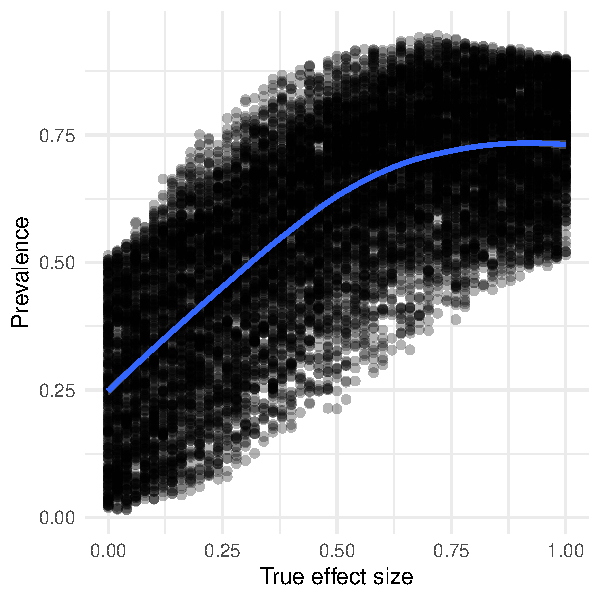
\includegraphics{../analysis/sim_fig.pdf}
\caption{\label{fig:simfig}The relationship between true effect size and observed prevalence of X. The line represents the local regression line}
\end{figure}

\begin{figure}
\centering
\includegraphics{paper_files/figure-latex/fixfig-1.pdf}
\caption{\label{fig:fixfig}The relationship between true negative rate (X-axis) and observed effect size (Y-axis) by true positive rate (column). The line represents the median of all simulated observed effect sizes and the ribbon represents its 95\% interval estimation.}
\end{figure}

Also drawing from medical research, the Standards for Reporting Diagnostic Accuracy (STARD) statement mandates the reporting of \enquote{Cross tabulation of the index test results (or their distribution) by the results of the reference standard} and \enquote{Estimates of diagnostic accuracy and their precision} (Bossuyt et al., 2015). Therefore, a medical diagnostic study needs to report accuracy metrics, their precision (e.g.~95\% Confidence Interval), and cross tabulations (See this paper for an example: Prince-Guerra et al., 2021). This practice should be ported to communication research.

The cross tabulation, which is called Confusion Matrix in machine learning literature, complements metrics. It is also more useful than the so-called heatmap visualization of Confusion Matrix because cross tabulation provides raw numbers, not just color depths. The numbers are important because they provide clues on whether the predictive accuracy data are subjected to random sampling error. A measurement of \(\zeta\) calculated with only a few cases is less accurate than the ones with a lot of cases. The provided R function \texttt{cal\_bigphi} also supports these numbers (the parameters \texttt{tpn}, \texttt{tnn}, \texttt{Qn}, the denominators for calculating \(\zeta_{+}\), \(\zeta_{-}\), and \(Q\) respectively) by assuming probabilities such as \(\zeta_{+}\), \(\zeta_{-}\), and \(Q\) are drawn from a binomial distribution, \(\mathcal{B}(n, p)\). When these probabilities are calculated with a larger sample size, they are more accurate and subjected to less random sampling error.

\begin{Shaded}
\begin{Highlighting}[]
\KeywordTok{cal_bigphi}\NormalTok{(}\DataTypeTok{rho =} \FloatTok{0.0852}\NormalTok{, }\DataTypeTok{n =} \DecValTok{2019}\NormalTok{,}
           \DataTypeTok{tpr =} \FloatTok{0.831}\NormalTok{, }\DataTypeTok{tnr =} \FloatTok{0.721}\NormalTok{,}
           \DataTypeTok{Q =} \FloatTok{0.8964}\NormalTok{, }\DataTypeTok{tpn =} \DecValTok{1000}\NormalTok{,}
           \DataTypeTok{tnn =} \DecValTok{300}\NormalTok{, }\DataTypeTok{Qn =} \DecValTok{400}\NormalTok{)}
\end{Highlighting}
\end{Shaded}

Regarding the number of cases for study \(Q\) and \(\zeta\), Song et al. (2020) advise researchers to \enquote{strive to increase the sizes of manually coded validation dataset as large as possible, preferably to more than N = 1,300 \ldots{}, assuming acceptable reliability (equal to or higher than .7)}. I agree with this advice in principle but it is also important to get enough positive and negative cases so that both \(\zeta_{+}\) and \(\zeta_{-}\) are accurate. However, this cannot be achieved by deliberately oversampling positive or negative cases, because of the problem below.

\hypertarget{rule-out-systematic-measurement-error}{%
\subsection{3. Rule out systematic measurement error}\label{rule-out-systematic-measurement-error}}

It is also important to note that the subject matter in this paper is \emph{random} measurement error. And all the simulation conducted in this paper assumes that \emph{systematic} measurement error is negligible. As stated in the Introduction section, systematic measurement error could influence both the variance and the average level of a variable, but the direction of influence depends on the composition of data.

Unlike the Monte Carlo simulation, systematic measurement error exists in real life and it's not common for (communication) researchers to report it. In a methodological research, Song et al. (2020) study one source of systematic measurement error: the non-random selection of cases for validating prediction models and such practice will generate bias in the estimation of \(\zeta\). Therefore, it is inappropriate to oversample positive or negative cases to achieve higher \(n\) in the validation procedure. \(P(X)\) should be kept like the natural distribution in the entire dataset. Therefore, the valid way to increase the number of positive and negative cases is to increase the number of random samples, not deliberately select more positive or negative cases.

The composition of the cases for conducting the validation procedure is not the only source of systematic measurement error. Sometimes the error is not straightforward to detect and needs to be detected qualitatively. I recommend the error analysis process as in Van Atteveldt et al. (2021) to qualitatively document what kind of cases got misclassified.

\hypertarget{coda}{%
\section{Coda}\label{coda}}

The entry point for automated content analysis is to scale up content analysis for the ever-increasing size of datasets (Lewis, Zamith, \& Hermida, 2013; Trilling \& Jonkman, 2018). In other words, automated content analysis allows researchers to \emph{ob}tain more statistical power through increasing \emph{n} and to study some extremely small effect sizes without the risk of Type II error. The findings from this study, however, underscores the problem in \emph{re}tain those obtained statistical power due to the automation-induced measurement errors. When we do not look at the problem in terms of statistical power, which is only relevant to the frequentist inference, the ACIDIC problem underestimates effect sizes.

Obtaining more statistical power and obtaining unbiased effect sizes are like weddings. One cannot dance at two weddings at the same time.

\hypertarget{references}{%
\section{References}\label{references}}

\begingroup
\setlength{\parindent}{-0.5in}
\setlength{\leftskip}{0.5in}

\hypertarget{refs}{}
\leavevmode\hypertarget{ref-bachl:2017:CME}{}%
Bachl, M., \& Scharkow, M. (2017). Correcting measurement error in content analysis. \emph{Communication Methods and Measures}, \emph{11}(2), 87--104. \url{https://doi.org/10.1080/19312458.2017.1305103}

\leavevmode\hypertarget{ref-barberuxe1:2020:atc}{}%
Barberá, P., Boydstun, A. E., Linn, S., McMahon, R., \& Nagler, J. (2020). Automated text classification of news articles: A practical guide. \emph{Political Analysis}, 1--24. \url{https://doi.org/10.1017/pan.2020.8}

\leavevmode\hypertarget{ref-bossuyt:2015:S}{}%
Bossuyt, P. M., Reitsma, J. B., Bruns, D. E., Gatsonis, C. A., Glasziou, P. P., Irwig, L., \ldots{} Cohen, J. F. (2015). STARD 2015: An updated list of essential items for reporting diagnostic accuracy studies. \emph{BMJ}, h5527. \url{https://doi.org/10.1136/bmj.h5527}

\leavevmode\hypertarget{ref-chan:2020:REC}{}%
Chan, C.-h., Zeng, J., Wessler, H., Jungblut, M., Welbers, K., Bajjalieh, J. W., \ldots{} Althaus, S. L. (2020). Reproducible extraction of cross-lingual topics (rectr). \emph{Communication Methods and Measures}, 1--21. \url{https://doi.org/10.1080/19312458.2020.1812555}

\leavevmode\hypertarget{ref-chicco:2020:MMF}{}%
Chicco, D., \& Jurman, G. (2020). The advantages of the matthews correlation coefficient (MCC) over F1 score and accuracy in binary classification evaluation. \emph{BMC Genomics}, \emph{21}(1). \url{https://doi.org/10.1186/s12864-019-6413-7}

\leavevmode\hypertarget{ref-corliss:1977:WRD}{}%
Corliss, G. (1977). Which root does the bisection algorithm find? \emph{SIAM Review}, \emph{19}(2), 325--327. \url{https://doi.org/10.1137/1019044}

\leavevmode\hypertarget{ref-dimaggio:2013:E}{}%
DiMaggio, P., Nag, M., \& Blei, D. (2013). Exploiting affinities between topic modeling and the sociological perspective on culture: Application to newspaper coverage of u.s. Government arts funding. \emph{Poetics}, \emph{41}(6), 570--606. \url{https://doi.org/10.1016/j.poetic.2013.08.004}

\leavevmode\hypertarget{ref-dobbrick:2021:ETI}{}%
Dobbrick, T., Jakob, J., Chan, C.-H., \& Wessler, H. (2021). Enhancing theory-informed dictionary approaches with ``glass-box'' machine learning: The case of integrative complexity in social media comments. \emph{Communication Methods and Measures}, 1--18. \url{https://doi.org/10.1080/19312458.2021.1999913}

\leavevmode\hypertarget{ref-ethayarajh2020utility}{}%
Ethayarajh, K., \& Jurafsky, D. (2020). Utility is in the eye of the user: A critique of NLP leaderboards. \emph{arXiv Preprint arXiv:2009.13888}.

\leavevmode\hypertarget{ref-frost:2000:C}{}%
Frost, C., \& Thompson, S. G. (2000). Correcting for regression dilution bias: Comparison of methods for a single predictor variable. \emph{Journal of the Royal Statistical Society: Series A (Statistics in Society)}, \emph{163}(2), 173--189. \url{https://doi.org/10.1111/1467-985x.00164}

\leavevmode\hypertarget{ref-fuller2009measurement}{}%
Fuller, W. A. (2009). \emph{Measurement error models}. John Wiley \& Sons.

\leavevmode\hypertarget{ref-geiss2021statistical}{}%
Geiß, S. (2021). Statistical power in content analysis designs. \emph{Computational Communication Research}, \emph{3}(1), 61--89. \url{https://doi.org/10.5117/CCR2021.1.003.GEIß}

\leavevmode\hypertarget{ref-gerring:2012:MD}{}%
Gerring, J. (2012). Mere description. \emph{British Journal of Political Science}, \emph{42}(4), 721--746. \url{https://doi.org/10.1017/s0007123412000130}

\leavevmode\hypertarget{ref-gilardi:2021:SMP}{}%
Gilardi, F., Gessler, T., Kubli, M., \& Müller, S. (2021). Social media and political agenda setting. \emph{Political Communication}, \emph{39}(1), 39--60. \url{https://doi.org/10.1080/10584609.2021.1910390}

\leavevmode\hypertarget{ref-GonzlezBailn2015}{}%
González-Bailón, S., \& Paltoglou, G. (2015). Signals of public opinion in online communication. \emph{The ANNALS of the American Academy of Political and Social Science}, \emph{659}(1), 95--107. \url{https://doi.org/10.1177/0002716215569192}

\leavevmode\hypertarget{ref-Grimmer2013}{}%
Grimmer, J., \& Stewart, B. M. (2013). Text as data: The promise and pitfalls of automatic content analysis methods for political texts. \emph{Political Analysis}, \emph{21}(3), 267--297. \url{https://doi.org/10.1093/pan/mps028}

\leavevmode\hypertarget{ref-guo:2019:AFB}{}%
Guo, L., Mays, K., Lai, S., Jalal, M., Ishwar, P., \& Betke, M. (2019). Accurate, fast, but not always cheap: Evaluating ``crowdcoding'' as an alternative approach to analyze social media data. \emph{Journalism \& Mass Communication Quarterly}, \emph{97}(3), 811--834. \url{https://doi.org/10.1177/1077699019891437}

\leavevmode\hypertarget{ref-hayden:1999:LR}{}%
Hayden, S. R., \& Brown, M. D. (1999). Likelihood ratio: A powerful tool for incorporating the results of a diagnostic test into clinical decisionmaking. \emph{Annals of Emergency Medicine}, \emph{33}(5), 575--580. \url{https://doi.org/10.1016/s0196-0644(99)70346-x}

\leavevmode\hypertarget{ref-hutcheon:2010:R}{}%
Hutcheon, J. A., Chiolero, A., \& Hanley, J. A. (2010). Random measurement error and regression dilution bias. \emph{BMJ}, \emph{340}(jun23 2), c2289--c2289. \url{https://doi.org/10.1136/bmj.c2289}

\leavevmode\hypertarget{ref-knox:2022:TCT}{}%
Knox, D., Lucas, C., \& Cho, W. K. T. (2022). Testing causal theories with learned proxies. \emph{Annual Review of Political Science}, \emph{25}(1). \url{https://doi.org/10.1146/annurev-polisci-051120-111443}

\leavevmode\hypertarget{ref-krippendorff:2011:AIR}{}%
Krippendorff, K. (2011). Agreement and information in the reliability of coding. \emph{Communication Methods and Measures}, \emph{5}(2), 93--112. \url{https://doi.org/10.1080/19312458.2011.568376}

\leavevmode\hypertarget{ref-krippendorff2018content}{}%
Krippendorff, K. (2018). \emph{Content analysis: An introduction to its methodology}. SAGE.

\leavevmode\hypertarget{ref-lacy:2015:IBP}{}%
Lacy, S., Watson, B. R., Riffe, D., \& Lovejoy, J. (2015). Issues and best practices in content analysis. \emph{Journalism \& Mass Communication Quarterly}, \emph{92}(4), 791--811. \url{https://doi.org/10.1177/1077699015607338}

\leavevmode\hypertarget{ref-lewis:2013:CAE}{}%
Lewis, S. C., Zamith, R., \& Hermida, A. (2013). Content analysis in an era of big data: A hybrid approach to computational and manual methods. \emph{Journal of Broadcasting \&Amp; Electronic Media}, \emph{57}(1), 34--52. \url{https://doi.org/10.1080/08838151.2012.761702}

\leavevmode\hypertarget{ref-osborne:2002:ESD}{}%
Osborne, J. W. (2002). \emph{Effect sizes and the disattenuation of correlation and regression coefficients: Lessons from educational psychology}. \url{https://doi.org/10.7275/0K9H-TQ64}

\leavevmode\hypertarget{ref-prince-guerra:2021:EAB}{}%
Prince-Guerra, J. L., Almendares, O., Nolen, L. D., Gunn, J. K. L., Dale, A. P., Buono, S. A., \ldots{} Bower, W. A. (2021). Evaluation of Abbott BinaxNOW Rapid Antigen Test for SARS-CoV-2 Infection at Two Community-Based Testing Sites --- Pima County, Arizona, November 3--17, 2020. \emph{MMWR. Morbidity and Mortality Weekly Report}, \emph{70}(3), 100--105. \url{https://doi.org/10.15585/mmwr.mm7003e3}

\leavevmode\hypertarget{ref-rains:2018:S}{}%
Rains, S. A., Levine, T. R., \& Weber, R. (2018). Sixty years of quantitative communication research summarized: Lessons from 149 meta-analyses. \emph{Annals of the International Communication Association}, \emph{42}(2), 105--124. \url{https://doi.org/10.1080/23808985.2018.1446350}

\leavevmode\hypertarget{ref-raji2021ai}{}%
Raji, I. D., Bender, E. M., Paullada, A., Denton, E., \& Hanna, A. (2021). AI and the everything in the whole wide world benchmark. \emph{arXiv Preprint arXiv:2111.15366}.

\leavevmode\hypertarget{ref-song:2020:ivw}{}%
Song, H., Tolochko, P., Eberl, J.-M., Eisele, O., Greussing, E., Heidenreich, T., \ldots{} Boomgaarden, H. G. (2020). In validations we trust? The impact of imperfect human annotations as a gold standard on the quality of validation of automated content analysis. \emph{Political Communication}, \emph{37}(4), 550--572. \url{https://doi.org/10.1080/10584609.2020.1723752}

\leavevmode\hypertarget{ref-spearman:1904:PMA}{}%
Spearman, C. (1904). The proof and measurement of association between two things. \emph{The American Journal of Psychology}, \emph{15}(1), 72. \url{https://doi.org/10.2307/1412159}

\leavevmode\hypertarget{ref-su:2018:U}{}%
Su, L. Y.-F., Xenos, M. A., Rose, K. M., Wirz, C., Scheufele, D. A., \& Brossard, D. (2018). Uncivil and personal? Comparing patterns of incivility in comments on the facebook pages of news outlets. \emph{New Media \&Amp; Society}, \emph{20}(10), 3678--3699. \url{https://doi.org/10.1177/1461444818757205}

\leavevmode\hypertarget{ref-trilling:2018:SCA}{}%
Trilling, D., \& Jonkman, J. G. F. (2018). Scaling up content analysis. \emph{Communication Methods and Measures}, \emph{12}(2-3), 158--174. \url{https://doi.org/10.1080/19312458.2018.1447655}

\leavevmode\hypertarget{ref-upton2014}{}%
Upton, G., \& Cook, I. (2014). \emph{A dictionary of statistics 3e}. Oxford university press.

\leavevmode\hypertarget{ref-atteveldt:2018:wcm}{}%
Van Atteveldt, W., \& Peng, T.-Q. (2018). When communication meets computation: Opportunities, challenges, and pitfalls in computational communication science. \emph{Communication Methods and Measures}, \emph{12}(2-3), 81--92. \url{https://doi.org/10.1080/19312458.2018.1458084}

\leavevmode\hypertarget{ref-atteveldt:2021:VSA}{}%
Van Atteveldt, W., Velden, M. A. C. G. van der, \& Boukes, M. (2021). The validity of sentiment analysis:Comparing manual annotation, crowd-coding, dictionary approaches, and machine learning algorithms. \emph{Communication Methods and Measures}, 1--20. \url{https://doi.org/10.1080/19312458.2020.1869198}

\leavevmode\hypertarget{ref-western:1994:BIC}{}%
Western, B., \& Jackman, S. (1994). Bayesian inference for comparative research. \emph{American Political Science Review}, \emph{88}(2), 412--423. \url{https://doi.org/10.2307/2944713}

\leavevmode\hypertarget{ref-wickham:2010:G}{}%
Wickham, H., Cook, D., Hofmann, H., \& Buja, A. (2010). Graphical inference for infovis. \emph{IEEE Transactions on Visualization and Computer Graphics}, \emph{16}(6), 973--979. \url{https://doi.org/10.1109/tvcg.2010.161}

\leavevmode\hypertarget{ref-yule:1912:MMA}{}%
Yule, G. U. (1912). On the methods of measuring association between two attributes. \emph{Journal of the Royal Statistical Society}, \emph{75}(6), 579. \url{https://doi.org/10.2307/2340126}

\endgroup


\end{document}
